\section{Adattamento di fase}

Si è realizzato il circuito in \fig{sfas_circ}, che ha in ultima analisi lo scopo di generare un'onda approssimativamente quadra della stessa frequenza del segnale inviato al LED e che abbia con esso una precisa relazione di fase.

\begin{figure}[h]
	\centering
	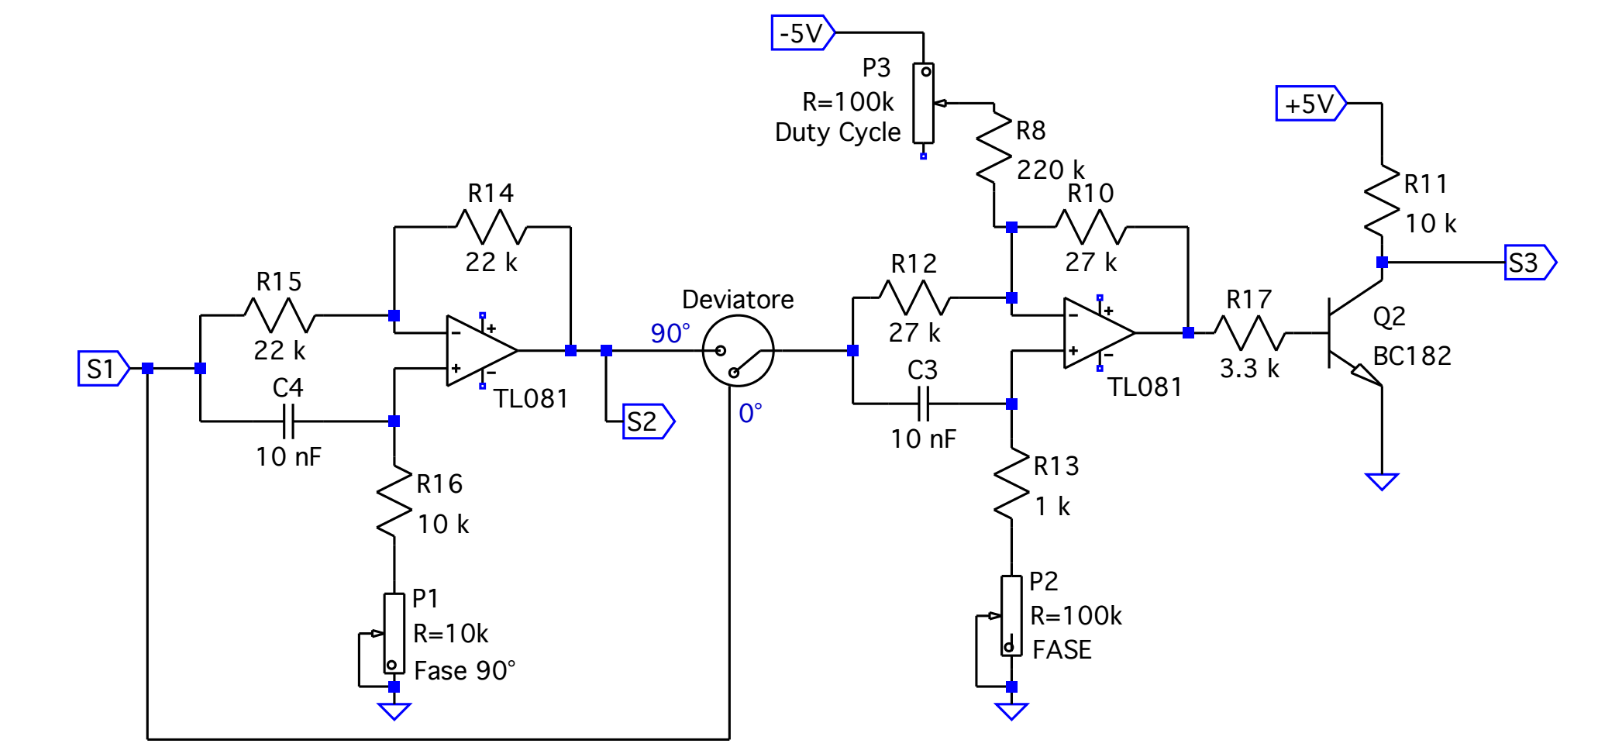
\includegraphics[scale=.35]{sfaso.png}
	\caption{Circuiti sfasatori (\ang{90} e fase variabile).}
	\label{fig:sfas_circ}
\end{figure}

\subsection{Sfasatore di \ang{90}}

Si vuole che la prima sezione del circuito (quella precedente al deviatore) introduca uno sfasamento di $\SI{\pi/2}{rad}$ nel segnale in ingresso; la sua funzione di trasferimento (determinata col metodo del cortocircuito virtuale) è:
$$ V_{S2} = \longfrac{j \omega C_4 (P_1 + R_{16}) R_{14} / R_{15} - 1}{j \omega C_4 (P_1 + R_{16}) + 1} \ V_{S1}  $$
Dove $P_1$ rappresenta l'effettiva resistenza nel potenziometro nella posizione usata.
La differenza di fase tra ingresso e uscita vale dunque:
$$ \phi_{S2} - \phi_{S1} = \Delta\phi_1 = \pi - \atan \left( \omega  C_4 (P_1 + R_{16}) \frac{R_{14}}{R_{15}} \right) - \atan\mathopen{}\big( \omega C_4 (P_1 + R_{16}) \mathclose{}\big)$$
Ed è dunque decrescente dal suo valore massimo al crescere di $P_1$. Si è pertanto proceduto a regolare il potenziometro ottenendo una differenza temporale tra $S1$ ed $S2$ pari a \SI{244(2)}{\us}, che alla frequenza di lavoro di \SI{1.026(2)}{\kHz} corrisponde ad una differenza di fase di \SI{0.498(2)}{\pie.rad}.

\subsection{Sfasatore a fase variabile e transistor NOT}

La seconda parte del circuito intende nuovamente sfruttare un OpAmp per introdurre una differenza di fase ed inoltre un offset; l'output dell'OpAmp andrà (attraverso una resistenza per limitare il flusso di corrente) alla base di un transistor BJT in configurazione common emitter, il quale ha essenzialmente un comportamento da NOT gate: l'offset è necessario per compensare la tensione di soglia (positiva) per la commutazione del transistor e permetterci di ottenere un duty cicle del \SI{50}{\percent}.

La relazione tra ingresso e uscita del circuito è:

$$ V_{out} = \longfrac{j \omega C_3 (P_2 + R_{13}) R_{10} \big(1/R_{12} + 1/(R_8 + P_3)\big) - 1}{j \omega C_3 (P_2 + R_{13}) + 1} \, V_{in} + \longfrac{R_{10}}{R_8 + P_3} \, \SI{5}{\V}$$

Dove $V_{in}$ è la tensione in corrispondenza del deviatore, $V_{out}$ la tensione in uscita all'OpAmp e $P_2$ e $P_3$ sono le effettive resistenze dei potenziometri nelle posizioni usate.

Si è dunque variato $P3$ in modo da ottenere in $S3$ un'onda quadra con $T_{up} = \SI{484(4)}{\us}$, essenzialmente pari alla metà del periodo dell'onda (\SI{987(1)}{\us}), riportata in \fig{duty_quadra}.

\begin{figure}[h]
	\centering
	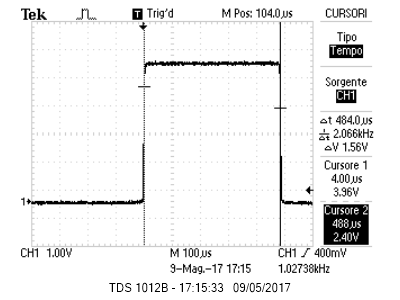
\includegraphics{duty_cycle.png}
	\caption{Segnale in uscita in $S3$.}
	\label{fig:duty_quadra}
\end{figure}

Il deviatore ci permette di avere in ingresso in quest'ultima sezione del circuito alternativamente il segnale inviato al LED oppure il segnale in uscita allo sfasatore di \ang{90}, consentendoci di introdurre a comando uno sfasamento di $\SI{\pi/2}{rad}$ nel segnale in uscita, che sarà necessario nel seguito dell'esperienza.
